\chapter{Design and Optimisation} 


\section{NAND}

\section{NOR2}

\section{XOR2}

\section{DFF}
The design goal for the DFF was high speed. Initially it was designed using a standard circuit composed of NAND gates. However then the option of Transmission gates was considered and found to be superior. Using transmission gates a master slave style flip plot was produced as shown in figure \ref{fig:DFFSchem}. A ratio between PMOS and NMOS of 3 was chosen as it is the integer ratio which produced the best results for rise and fall time matching. As 0.35$\mu$ is the length set by the technology used the only parameter used is NWIDTH for each gate as PWIDTH is simply 3 times that.

\begin{figure}[h]  
\centering
   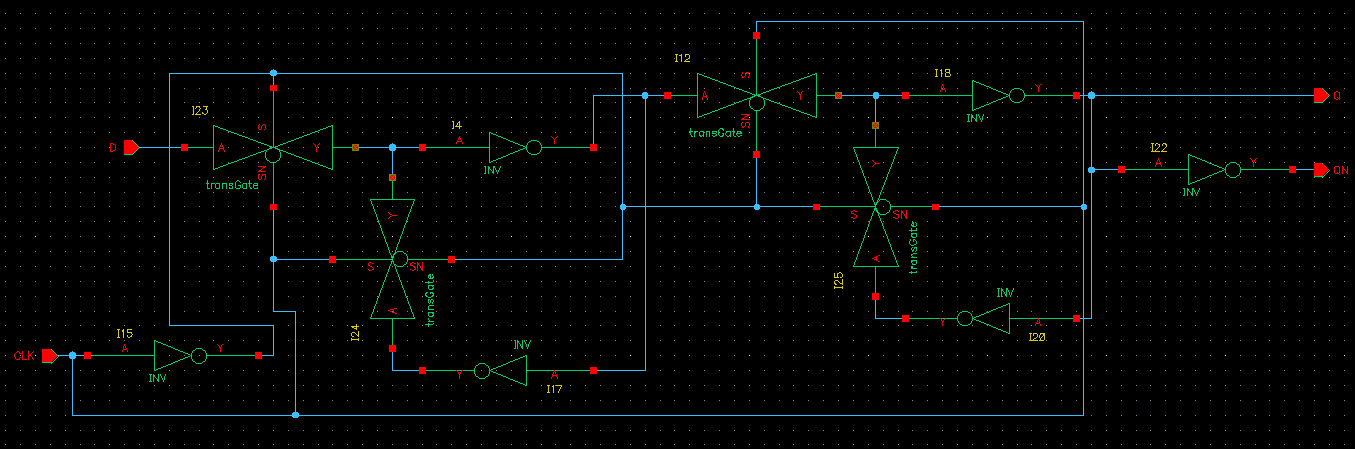
\includegraphics[width=0.45\textwidth]{Figures/DFFSchem.png}
\caption{DFF Schematic.}
\label {fig:DFFSchem}
\end{figure}

In terms of transistor sizes the Transmission gate and the Inverters were considered as separate parameters although there was only one size for each family This may have been a bad decision in terms of the inverter creating CLKN as it has to drive 4 components where as the maximum of any other gate was only 2, However in this situation it was not much of a problem as the relatively large transistor sizes chosen to deliver high speed negated much of this effect.

By using the rise times, as shown in figure \ref{fig:DDFNW}, among other metrics when measured in the test circuit Values for NMOS and PMOS widths were chosen based on giving maximum performance. These turned out to be a 11$\mu$m for the transmission gate and 17.5 $\mu$m for the inverter. This is quite large but as the only restriction on the design is that it must be high speed regardless of area.

\begin{figure}[h]
\centering
\subfigure[Inverter N Width]{
  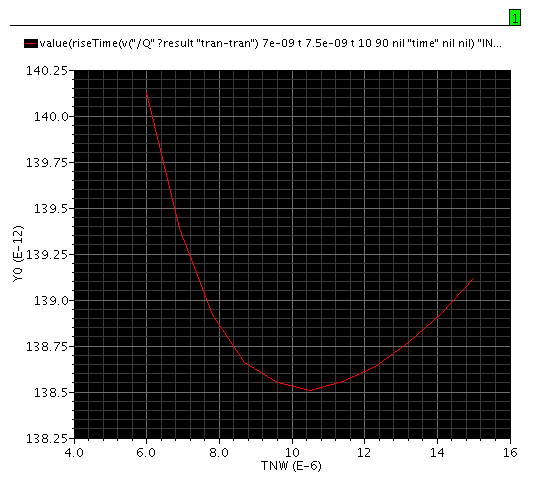
\includegraphics[width=.225\textwidth]{Figures/DFF1fFLoadTNW.png}
  \label{fig:DFFINW}}
\subfigure[Transmission gate N Width]{
  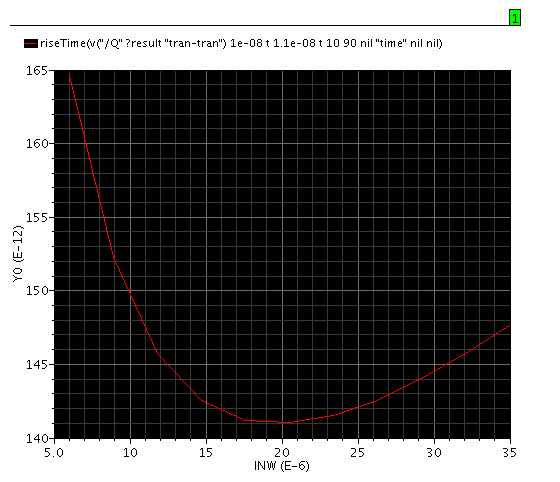
\includegraphics[width=.225\textwidth]{Figures/DFF1fFLoadINW.png}
  \label{fig:DDFTNW}}
\caption{Transistor size effect on rise time.}
\label{fig:DDFNW}
\end{figure}

One point of note is that the QN output is created via a separate inverter rather than taking the signal from either side of the left most transmission gate. This was because large capacitive loads on QN caused incorrect circuit behaviour as this effected the transition time across the transmission gate which incorrect circuit behaviour on extreme loads where the slave circuit wouldn't latch new master value.

\begin{figure}[h]  
\centering
   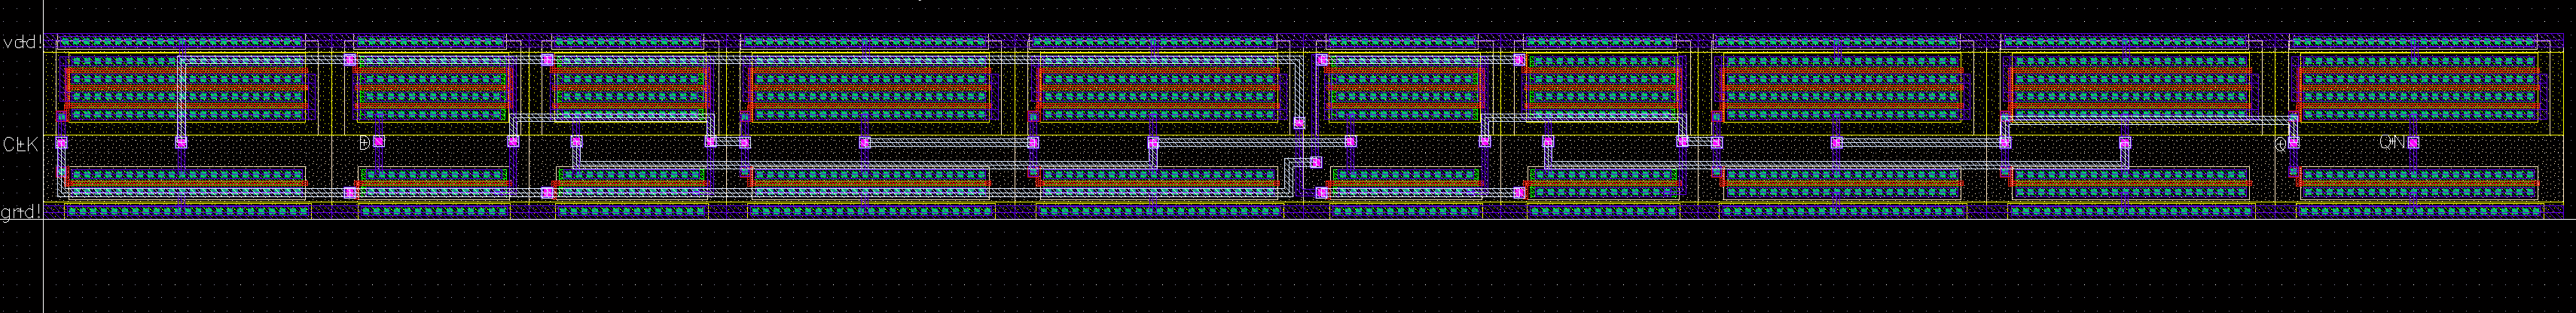
\includegraphics[width=0.45\textwidth]{Figures/DFFLayout.png}
\caption{DFF Layout.}
\label {fig:DFFLayout}
\end{figure}

Due to the large transistor size layout was not particularly difficult as there was a lot of space for gate interconnects. When laying out the gates were placed in an order such as to minimise local process variations however with such large gates this is not particularly effective. A future layout revision could increase robustness by splitting the transistors into 2 or 3 smaller transistors of equal total size and interleaving them.

\section{Duel Edge Triggered Flip Flop}

The Dual Edge Triggered Flip Flop (DETFF) was designed using transmission gates as this allows the design to contain a minimum of 20 transistors (18 if there is no requirement for QN). Figure \ref{fig:DETFFSchem} shows the schematic produced. A ratio between PMOS and NMOS of 3 was chosen as it is the integer ratio which produced the best results for rise and fall time matching. As 0.35$\mu$ is the length set by the technology used the only parameter used is NWIDTH for each gate as PWIDTH is 3 times that.

\begin{figure}[h]  
\centering
   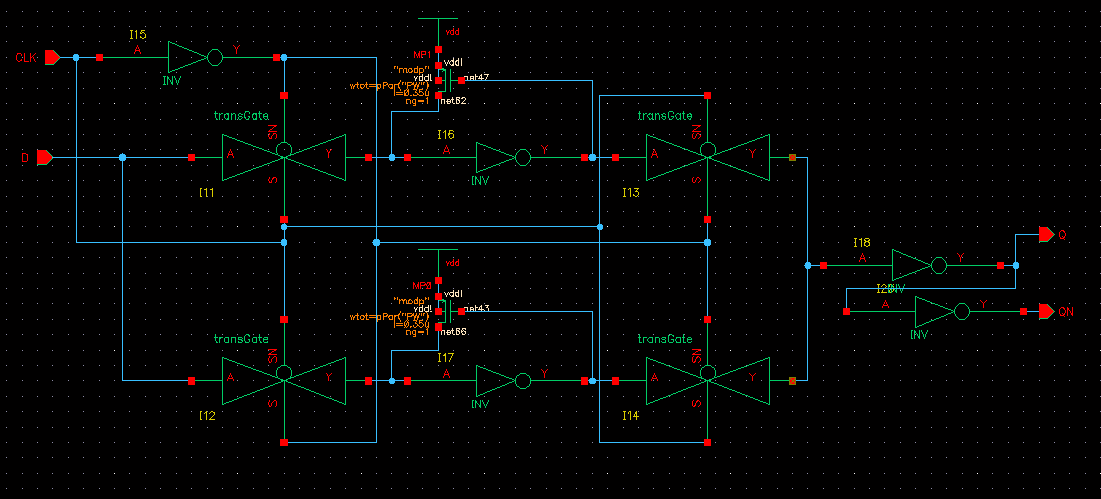
\includegraphics[width=0.45\textwidth]{Figures/DETFFSchem.png}
\caption{DETFF Schematic.}
\label {fig:DETFFSchem}
\end{figure}

The size of the gates where considered in terms of Transmission gates NMOS Width, Inverters NMOS Width and the 2 PMOS pull up transistors width. These parameters were brought to minimum  values of 1.2$\mu$m 2$\mu$m and 4$\mu$m (Trans NW,Inv NW,Pwidth respectively) before correct operation ceased. However these values were found to be to small for effective layout without enough space for interconnects and routing to fit due to DRC constraints, they also gave speed performance deemed unacceptable. The sizes were increased until sensible routing and speed was achieved  at values of 2.4$\mu$m 3.2$\mu$m and 4.7$\mu$m (Trans NW,Inv NW,Pwidth respectively).

\begin{figure}[h]  
\centering
   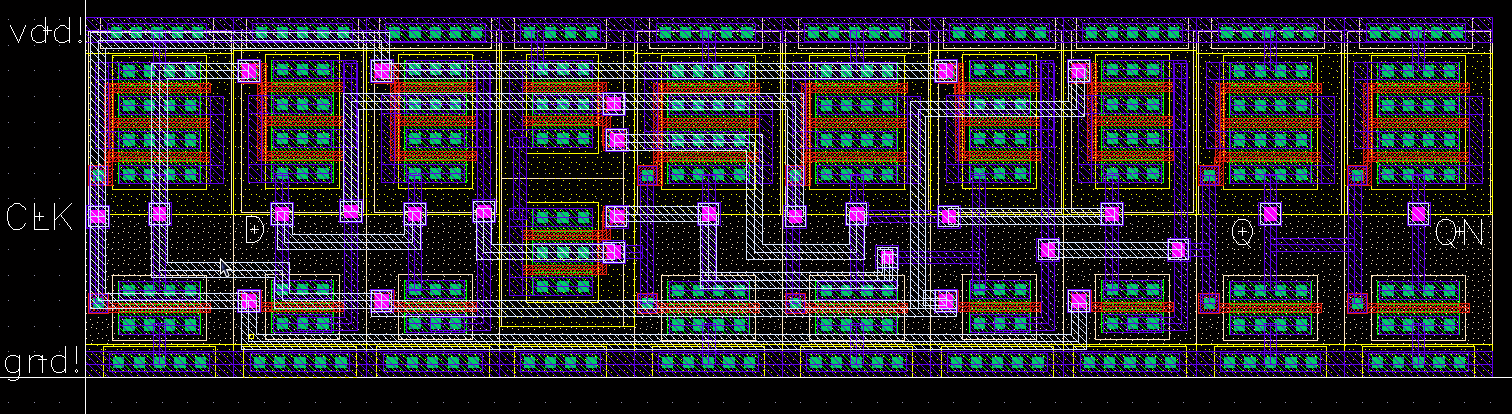
\includegraphics[width=0.45\textwidth]{Figures/DETFFLayout.png}
\caption{DETFF Layout.}
\label {fig:DETFFLayout}
\end{figure}

Figure \ref{fig:DETFFLayout} shows the final layout of the DETFF its easily visible that this is towards the limit of gate size for the given layout in particular in crowded areas such as the between gates 6 and 7. The option of using MET3 in this area was considered but it was not specified this layer was available for use also as a consideration to real world manufacture having to add another metal layer because of a single gate when a 2 layer design is possible would not be viable.

The layout of the design initial versions of the Transmission and inverter were lain out  at the minimum possible width and copied to populate the design and as interconnects were placed some of them had the wells expanded to allow for interconnect spacing.The pull-up PMOS are stacked vertically so as to not waste horizontal space as the rail distance is fixed meaning total area is effected by the width of the entire gate.

\section{C Element}

\section{Dual Rail AND}
The design goal for the Dual Rail AND was small area. The design was chosen based on its simplicity and the fact that the C-Element had the same goal of small area. This fact allowed us to simply reuse the C-Element with fixed parameters and reuse its layout saving substantial amounts of work in layout. there is a disparity between the Required fan-outs however as the fanout of the c-element is two and the AND has a fanout of one meaning the extra area gained is not too great.

\begin{figure}[h]  
\centering
   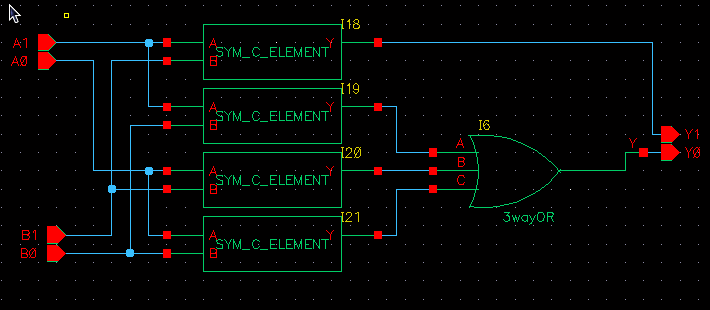
\includegraphics[width=0.45\textwidth]{Figures/DualRailANDSchem.png}
\caption{Dual Rail AND Schematic.}
\label {fig:DualRailANDSchem}
\end{figure}

The only element in this design that required optimisation in design was the 3 input OR gate. This was constructed from a 3 input NOR gate and an inverter on the output. The PMOS and NMOS ratio was set at 3 and the characteristics matched to that of the output of the C-element meaning there should be minimum disparity between the Y0 and Y1 signals. The Nwidth was finalised at 4$\mu$m This is slightly larger than is strictly necessary but helps reduce the propagation disparity between the outputs.



\section{1-bit Subtractor}

\section{2-to-1 Multiplexor}

\section{Mutex Element}
